\section{Relevant Model Details}

A brief overview of the salient features of the HuMoR model and TestOps optimisation procedure is provided here, some details are ommited for clarity and brevity.

\subsection{Architecture}
The HuMoR architecture is that of a C-VAE \cite{CVAE}, as can be seen in \figref{fig:humor_architecture}. The goal of this architecture is to learn a mapping from a given pose ($\mathbf{x}_{t-1}$) to a distribution over latent transitions to the next pose (the $\textbf{\textcolor{orange}{prior}}$), and a mapping from a latent transition sampled from this distribution to a change in pose ($\textbf{\textcolor{RoyalBlue}{decoder}}$) that can be used to obtain the next state . This is achieved during training through an additional $\textbf{\textcolor{ForestGreen}{encoder}}$ that has the full information of the next state ($\textbf{x}_t$) also available to it, such that it can find the ideal latent transition, and therefore is used to guide the training of the $\textbf{\textcolor{orange}{prior}}$.

The networks operate on states, $\mathbf{x}_t$, consisting of a root translation, root orientation, 3D joint positions, and all their respective velocities, and additionally joint angles. This rich and redundant state representation is a superset of the SMPL models' state \cite{SMPL} (given some shape parameters $\beta$ required by SMPL).

\begin{figure}[!ht]
    \centering
    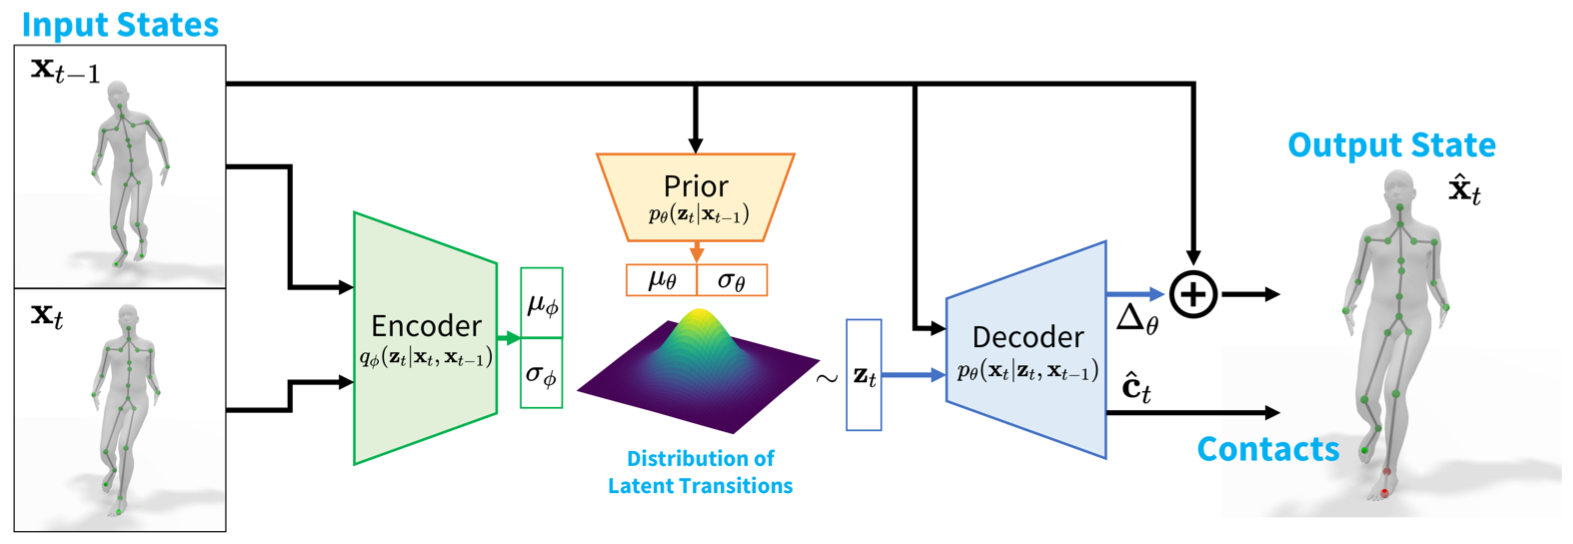
\includegraphics[width=1\textwidth]{Figures/humor/model/architecture.png}
    \caption{HuMoR C-VAE Architecture \cite{humor}}
    \label{fig:humor_architecture}
\end{figure}


\subsection{TestOps}
\label{sec:humor_test_ops}

\textbf{TestOps} is the term given by the authors of HuMoR to their method of using the HuMoR model in an optimisation procedure to obtain a smooth motion estimation from, among other things, an RGB video (our focus).

The concept of an autoregressive 'rollout' is important here. As we can see in \figref{fig:humor_architecture}, the model output can be used to obtain a new state. This new state can then be autoregressively fed back into the $\textbf{\textcolor{RoyalBlue}{decoder}}$, alongside either a given latent transition or one obtain through the $\textbf{\textcolor{orange}{prior}}$, to obtain the next state. The procedure of starting from a given state $\mathbf{x}_0$, and with a given sequence of latent transitions $\textbf{z}_{1:T}$, obtaining a sequence of states $\mathbf{x}_{1:T}$ through the autoregressive application of the HuMoR model is called a \textbf{rollout}.

The TestOps procedure is as follows for RGB video. First, frame by frame pose estimation is performed using OpenPose \cite{openPose} to obtain a 2d pose estimates. Next, a three stage optimisation procedure is proposed. The first two stages are used to obtain a data that can be used to get a rough estimate of input to the final stage, being an initial state $\mathbf{x}_0$ and a sequence of latent transitions $\textbf{z}_{1:T}$. The third stage then refines this estimate using the HuMoR model and outputs a polished sequence of states $\textbf{x}_{0:T}$.

\subsubsection{Stage 1}
The global root translation and orientation (in 3d space) is optimised using a loss comparing their projection to the 2d pose estimates. This is a small subset of the full state, and is optimised first so that we don't try and do too much, too soon.

\subsubsection{Stage 2}
\label{sec:humor_stage_2}
Next, the joint positions and angles are optimised (without the root) through the use of a projection loss to the 2d pose estimates, and of a number of regulariser losses, including smoothness and foot contact losses. An additional pose prior loss is included in this stage that ensures plausible poses using the VPoser \cite{VPoser} model. 

\subsubsection{Stage 3 (Initialisation)}
Using the root translation and orientation from Stage 1, and the joint positions from stage 2, the velocities of each of these elements can be calculated through finite differences, and all the variables, alongside the joint angles, can be considered the initial estimate $\mathbf{x}_{0:T}$ for the sequence of states. The initial estimates $\mathbf{x}_{0:T}$ are then fed through the $\textbf{\textcolor{ForestGreen}{encoder}}$ network to obtain initial estimates of the state transitions $\textbf{z}_{1:T}$.

\subsubsection{Stage 3 (Optimisation)}
The final optimisation then operates on a starting state $\mathbf{x}_0$, and a sequence of latent transitions $\textbf{z}_{1:T}$. For each optimisation step, a rollout (as described above) is performed to obtain a sequence of states $\mathbf{\hat{x}}_{1:T}$, and various losses are applied to these states. The regularisers as described in \secref{sec:humor_stage_2} are applied, a reprojection loss to the 2d pose estimates is used, and finally the HuMoR prior is used to evaluate the likelihood of each transition given the previous state. These losses are summed and the gradients are propagated back to the optimisation variables, $\mathbf{x}_0$ and $\textbf{z}_{1:T}$. This procedure is repeated for a number of steps, and a sequence of states $\mathbf{\hat{x}}_{0:T}$ is returned after a final rollout.


\subsubsection{Extra Notes}
\label{sec:humor_testops_extra_notes}

The computation graph entailed by this Stage 3 procedure is discussed later and can be seen in \figref{fig:humor_rollout_graph}.

Please note that some extra parameters are also optimised during this whole procedure, notably the ground plane and SMPL shape parameters, and a loss on the initial state $\mathbf{x}_0$ using a learned gaussian mixture model is applied during stage 3. The details however are not included as they are not vital to the investigation nor to the understanding of the important components of the method.